\documentclass[12pt,a4paper]{article}
\usepackage[utf8]{vietnam}
\usepackage{amsmath,amssymb}
\usepackage{tabularx}
\usepackage{tikz}
\usetikzlibrary{calc,angles,quotes,arrows.meta,patterns}
\usepackage{xcolor}
\usepackage{enumitem}
\usepackage{fancyhdr}
\usepackage{graphicx}
\usepackage[top=0.9cm, bottom=0.9cm, left=1.2cm, right=1.2cm]{geometry}
\usepackage[dethi]{ex_test}
\SAOPTN{widthSA=3.2,heightSA=0.62}

\setlength{\headheight}{15pt}
\setlength{\parskip}{0pt}

\pagestyle{fancy}
\fancyhf{}
\rhead{\textit{Môn Toán 8 -- Đề số 01}}
\lhead{\textit{Bộ đề ôn tập Giữa học kì I}}
\cfoot{\thepage}

\begin{document}

% --- KHUNG TIÊU ĐỀ ĐỀ THI ---
\noindent
\begin{tabularx}{\linewidth}{X r}
\textbf{TRƯỜNG THCS: \dotfill} & \textbf{ĐỀ KIỂM TRA ĐỊNH KỲ GIỮA HỌC KỲ I} \\
\textbf{Họ và tên: \dotfill} & \textbf{NĂM HỌC 2026 -- 2027} \\
\textbf{Lớp: \dotfill \quad SBD: \dotfill} & \textbf{Môn: TOÁN 8} \\
\hline
\end{tabularx}
\vspace{2mm}

\begin{center}
  \textbf{\large ĐỀ ÔN TẬP GIỮA HỌC KỲ I -- ĐỀ SỐ 01}\\
  \textit{Thời gian làm bài: 90 phút (Không kể thời gian phát đề)}
\end{center}
\vspace{1mm}

% --- PHẦN I ---
\noindent\textbf{\large PHẦN I. CÂU TRẮC NGHIỆM NHIỀU PHƯƠNG ÁN LỰA CHỌN (3,0 điểm)}

\textit{Thí sinh trả lời từ câu 1 đến câu 12. Mỗi câu hỏi thí sinh chỉ chọn một phương án duy nhất.}

\vspace{1mm}
\begin{ex}
Biểu thức nào sau đây là đơn thức?
\choice
{\True $5x^2y$}
{$2xy + 1$}
{$3x - 2$}
{$x^2 + 7$}
\end{ex}

\begin{ex}
Đơn thức đồng dạng với đơn thức $5x^3yz$ là:
\choice
{$-30x^2yz$}
{\True $x^3yz$}
{$-30xyz$}
{$40x^3y^5z$}
\end{ex}

\begin{ex}
Bậc của đa thức $A = 5x^3yz + \dfrac{1}{2}xy - 0{,}5x^4y^2$ là:
\choice
{3}
{4}
{5}
{\True 6}
\end{ex}

\begin{ex}
Cho hình chóp tam giác đều $A.BCD$ như hình vẽ bên. Đoạn thẳng nào sau đây là trung đoạn của hình chóp?
\begin{center}
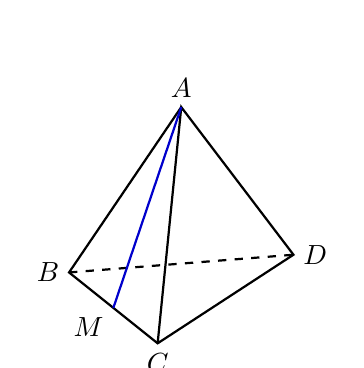
\begin{tikzpicture}[scale=0.75, baseline=(current bounding box.center)]
  \coordinate (B) at (0,0);
  \coordinate (D) at (3.8,0.3);
  \coordinate (C) at (1.5,-1.2);
  \coordinate (A) at (1.9,2.8);
  \coordinate (M) at ($(B)!0.5!(C)$);
  \draw[thick] (A) -- (B) -- (C) -- (D) -- (A) -- (C);
  \draw[dashed, thick] (B) -- (D);
  \draw[thick, blue!80!black] (A) -- (M);
  \node[above] at (A) {$A$};
  \node[left] at (B) {$B$};
  \node[below] at (C) {$C$};
  \node[right] at (D) {$D$};
  \node[below left] at (M) {$M$};
\end{tikzpicture}
\end{center}
\choice
{$AC$}
{\True $AM$}
{$BN$}
{$AP$}
\end{ex}

\begin{ex}
Tổng các góc của một tứ giác lồi bằng:
\choice
{\True $360^\circ$}
{$180^\circ$}
{$270^\circ$}
{$120^\circ$}
\end{ex}

\begin{ex}
Giá trị của biểu thức $x^3 - 3x^2 + 3x - 1$ tại $x = 2$ là:
\choice
{0}
{\True 1}
{2}
{16}
\end{ex}

\begin{ex}
Kết quả của phép tính $\dfrac{a - 2}{a - b} - \dfrac{2 - b}{b - a}$ là:
\choice
{$-1$}
{\True 1}
{$\dfrac{a - b}{b - a}$}
{$\dfrac{a + b - 4}{a - b}$}
\end{ex}

\begin{ex}
Cho tam giác $ABC$ vuông tại $A$ có $AB = 3\text{ cm}, AC = 4\text{ cm}$. Độ dài cạnh $BC$ bằng:
\choice
{\True $5\text{ cm}$}
{$6\text{ cm}$}
{$7\text{ cm}$}
{$8\text{ cm}$}
\end{ex}

\begin{ex}
Hình chữ nhật là tứ giác có:
\choice
{\True 4 góc vuông}
{2 góc kề một cạnh bằng nhau}
{2 góc kề một cạnh cùng bằng $90^\circ$}
{2 góc kề một cạnh bù nhau}
\end{ex}

\begin{ex}
Hình bình hành có hai cạnh kề bằng nhau là hình gì?
\choice
{Hình chữ nhật}
{Hình vuông}
{\True Hình thoi}
{Hình thang}
\end{ex}

\begin{ex}
Cho hình thang cân $ABCD$ có $AB \parallel CD$ và $\widehat{A} = 125^\circ$. Số đo của $\widehat{C}$ là:
\choice
{$125^\circ$}
{$65^\circ$}
{$90^\circ$}
{\True $55^\circ$}
\end{ex}

\begin{ex}
Tìm khẳng định sai trong các khẳng định sau:
\choice
{Hình chữ nhật có hai cạnh kề bằng nhau là hình vuông}
{Hình chữ nhật có hai đường chéo vuông góc là hình vuông}
{Hình chữ nhật có một đường chéo là đường phân giác của một góc vuông là hình vuông}
{\True Hình chữ nhật có bốn góc vuông là hình vuông}
\end{ex}


\vspace{1mm}
\noindent\textbf{BẢNG TRẢ LỜI TRẮC NGHIỆM PHẦN I:}
\begin{center}
\begin{tabular}{|c|c|c|c|c|c|c|c|c|c|c|c|c|}
\hline
\textbf{Câu} & \textbf{1} & \textbf{2} & \textbf{3} & \textbf{4} & \textbf{5} & \textbf{6} & \textbf{7} & \textbf{8} & \textbf{9} & \textbf{10} & \textbf{11} & \textbf{12} \\
\hline
\textbf{Chọn} & \rule{0pt}{0.65cm} & & & & & & & & & & & \\
\hline
\end{tabular}
\end{center}
\vspace{2mm}

\setcounter{ex}{0}
\noindent\textbf{\large PHẦN II. CÂU TRẮC NGHIỆM ĐÚNG SAI (2,0 điểm)}

\textit{Thí sinh trả lời câu 1 và câu 2. Trong mỗi ý a), b), c), d) ở mỗi câu, thí sinh chọn đúng hoặc sai.}

\vspace{1mm}
\begin{ex}
Cho hai đa thức $A = 3x^2y - 2xy^2 + 5$ và $B = x^2y + xy^2 - 1$. Xét tính đúng sai của các mệnh đề sau:
\choiceTF
{\True Bậc của đa thức $A$ bằng 3}
{\True Tổng của hai đa thức là $A + B = 4x^2y - xy^2 + 4$}
{Tại $x = 1$ và $y = -1$, giá trị của đa thức $B$ bằng 1}
{\True Tích của đa thức $A$ với đơn thức $2xy$ là $6x^3y^2 - 4x^2y^3 + 10xy$}
\end{ex}

\begin{ex}
Cho biểu thức $P = (x + 3)^2 - (x - 3)(x + 3)$ và đa thức $Q = x^3 - 4x$. Xét tính đúng sai của các mệnh đề sau:
\choiceTF
{\True Khai triển hằng đẳng thức $(x + 3)^2$ ta được $x^2 + 6x + 9$}
{\True Kết quả rút gọn của biểu thức $P$ là $6x + 18$}
{\True Phân tích đa thức $Q$ thành nhân tử ta được $x(x - 2)(x + 2)$}
{Tại $x = -3$, giá trị của biểu thức $P$ bằng 12}
\end{ex}


\noindent\textbf{BẢNG TRẢ LỜI PHẦN II:}
\begin{center}
\begin{tabular}{|c|c|c|c|c||c|c|c|c|c|}
\hline
\textbf{Câu 1} & \textbf{a)} & \textbf{b)} & \textbf{c)} & \textbf{d)} & \textbf{Câu 2} & \textbf{a)} & \textbf{b)} & \textbf{c)} & \textbf{d)} \\
\hline
\textbf{Đ/S} & \rule{0pt}{0.6cm} & & & & \textbf{Đ/S} & & & & \\
\hline
\end{tabular}
\end{center}
\vspace{2mm}

\setcounter{ex}{0}
\noindent\textbf{\large PHẦN III. CÂU HỎI TRẢ LỜI NGẮN (2,0 điểm)}

\textit{Thí sinh trả lời câu 1 và câu 2. Điền kết quả vào ô trống tương ứng.}

\vspace{1mm}
\begin{ex}
Cho hai đa thức $A = 2x^2y - 3xy + 5$ và $B = x^2y + 3xy - 2$. Tính $A + B$. \shortans{$3x^2y + 3$}
\end{ex}

\begin{ex}
Rút gọn biểu thức $P = (x + 3)^2 - (x - 3)(x + 3)$. \shortans{$6x + 18$}
\end{ex}


\setcounter{ex}{0}
\noindent\textbf{\large PHẦN IV. TỰ LUẬN (3,0 điểm)}

\textit{Thí sinh trình bày chi tiết lời giải vào giấy làm bài.}

\vspace{1mm}
\begin{ex} (2,0 điểm)
Thực hiện phép tính:
\begin{enumerate}[label=\textbf{\alph*)}, leftmargin=0.8cm, itemsep=2pt]
\item (0,5 điểm) $xy(x + y)$
\item (0,5 điểm) $(x - 2)^2 + 2x(x - 6)$
\item (1,0 điểm) $(2x^2 - 5xy - 4y^2)x - (2x^4y - 3x^3y^2 + 4x^2y^3) : xy$
\end{enumerate}
\end{ex}
\vspace{0.5mm}

\begin{ex} (1,5 điểm)
Phân tích các đa thức sau thành nhân tử:
\begin{enumerate}[label=\textbf{\alph*)}, leftmargin=0.8cm, itemsep=2pt]
\item (0,25 điểm) $4x^2 - 12x$
\item (0,25 điểm) $x^3 - 4x^2 + 4x$
\item (0,5 điểm) $x^2 - y^2 - 5x - 5y$
\item (0,5 điểm) $x^2 + 2xy + y^2 - 16$
\end{enumerate}
\end{ex}
\vspace{0.5mm}

\begin{ex} (1,0 điểm)
Cho tam giác $ABC$ vuông tại $A$ ($AB < AC$). Gọi $I$ là trung điểm của $BC$. Qua $I$ vẽ $IM \perp AB$ tại $M$, $IN \perp AC$ tại $N$.
\begin{center}
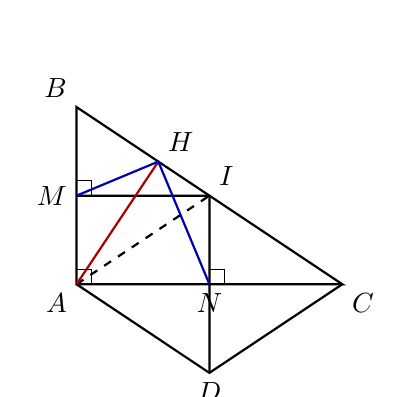
\begin{tikzpicture}[scale=0.75, baseline=(current bounding box.center)]
  \coordinate (A) at (0,0);
  \coordinate (B) at (0,3);
  \coordinate (C) at (4.5,0);
  \coordinate (I) at ($(B)!0.5!(C)$);
  \coordinate (M) at (0,1.5);
  \coordinate (N) at (2.25,0);
  \coordinate (D) at ($(N)!-1!(I)$);
  \coordinate (H) at ($(B)!(A)!(C)$);
  \draw[thick] (A) -- (B) -- (C) -- cycle;
  \draw[thick] (I) -- (M);
  \draw[thick] (I) -- (D);
  \draw[thick] (A) -- (D) -- (C);
  \draw[thick, dashed] (A) -- (I);
  \draw[thick, red!70!black] (A) -- (H);
  \draw[thick, blue!70!black] (M) -- (H) -- (N);
  \draw (0,0.25) -- (0.25,0.25) -- (0.25,0);
  \draw (0,1.75) -- (0.25,1.75) -- (0.25,1.5);
  \draw (2.25,0.25) -- (2.5,0.25) -- (2.5,0);
  \node[below left] at (A) {$A$};
  \node[above left] at (B) {$B$};
  \node[below right] at (C) {$C$};
  \node[above right] at (I) {$I$};
  \node[left] at (M) {$M$};
  \node[below] at (N) {$N$};
  \node[below] at (D) {$D$};
  \node[above right] at (H) {$H$};
\end{tikzpicture}
\end{center}
\begin{enumerate}[label=\textbf{\alph*)}, leftmargin=0.8cm, itemsep=2pt]
\item (0,5 điểm) Chứng minh rằng tứ giác $AMIN$ là hình chữ nhật.
\item (0,25 điểm) Lấy điểm $D$ trên tia đối của tia $NI$ sao cho $N$ là trung điểm của $ID$. Chứng minh tứ giác $ADCI$ là hình thoi.
\item (0,25 điểm) Kẻ $AH \perp BC$ tại $H$. Chứng minh $MH \perp HN$.
\end{enumerate}
\end{ex}
\vspace{0.5mm}

\begin{ex} (0,5 điểm)
Cho các số thực $x, y$ thỏa mãn điều kiện:
$$2x^2 + 10y^2 - 6xy - 6x - 2y + 10 = 0.$$
Tính giá trị của biểu thức $A = \dfrac{(x + y - 4)^{2018} - y^{2018}}{x}$.
\begin{enumerate}[label=\textbf{\alph*)}, leftmargin=0.8cm, itemsep=2pt]
\item (0,5 điểm) Tính giá trị biểu thức $A$.
\end{enumerate}
\end{ex}
\vspace{0.5mm}


\enlargethispage{1.5cm}
\begin{center}
\rule{4cm}{0.4pt}\\
\textit{--- HẾT ---}
\end{center}
\end{document}
